\section{Algorithm}

\subsection{Phase Wrapping}
Four phase-shifted sinusoidal fringes were used in the PSP experiment: 
\begin{align}
I_1(x,y)&=I_0(x,y) + I_{mod}(x,y)\cos{(\phi(x,y))}, \nonumber\\
I_2(x,y)&=I_0(x,y) + I_{mod}(x,y)\cos{(\phi(x,y)+\frac{\pi}{2})}, \nonumber\\
I_3(x,y)&=I_0(x,y) + I_{mod}(x,y)\cos{(\phi(x,y)+\pi)},\nonumber\\
I_4(x,y)&=I_0(x,y) + I_{mod}(x,y)\cos{(\phi(x,y)+\frac{3\pi}{2})},
\label{eq:four_fringes}
\end{align}  
where $I_0(x,y)$ is the average background intensity value, $I_{mod}(x,y)$ is the intensity value of the fringe pattern, and $I_i$, where $i=1,2,3,4$, is the intensity value of the $i^{th}$ image. To determine $I_0$ and $I_{mod}$, images of the fringes patterns projected to a reference plane and the actual object, respectively, are taken. 

To calculate the phase value $\phi(x,y)$, we express Eq.~(\ref{eq:four_fringes}) as 
\begin{align}
I_1(x,y)=I_0(x,y) + I_{mod}(x,y)\cos{(\phi(x,y))}, \nonumber\\
I_2(x,y)=I_0(x,y) - I_{mod}(x,y)\sin{(\phi(x,y))}, \nonumber\\
I_3(x,y)=I_0(x,y) - I_{mod}(x,y)\cos{(\phi(x,y))},\nonumber\\
I_4(x,y)=I_0(x,y) + I_{mod}(x,y)\sin{(\phi(x,y))}.
\label{eq:four_fringes2}
\end{align}  
Subtracting like terms, $I_2$ from $I_4$ and $I_3$ from $I_1$, we yield
\begin{align}
I_4(x,y)-I_2(x,y)&=2I_{mod}\sin{(\phi(x,y))}, \nonumber\\
I_1(x,y)-I_3(x,y)&=2I_{mod}\cos{(\phi(x,y))}.
\end{align}  
Dividing these two expressions, we get
\begin{equation}
\tan(\phi(x,y))=\frac{I_4-I_2}{I_1-I_3}.
\label{eq:tan_phase}
\end{equation}

Finally, the phase value is obtained by getting the inverse of Eq.~(\ref{eq:tan_phase}),
\begin{equation}
\phi(x,y)=\tan^{-1}{\left( \frac{I_4(x,y) - I_2(x,y)}{I_1(x,y)- I_3(x,y)}\right)}.
\label{eq:phase}
\end{equation}

Phase unwrapping is then performed to remove the discontinuities of the tangent inverse function at values near $2\pi$ by adding or subtracting multiples of $2\pi$.

\subsection{Phase Unwrapping}

Quality-guided path unwrapping algorithm by Herraez et al was implemented for efficient phase unwrapping \cite{Herraez2002}. 
MATLAB's built-in \texttt{unwrap} function was used by Vergara \cite{Vergara2010} in his thesis (2010) which he turned into a Graphical User Interface (GUI) consequently used by Sze \cite{Sze2012} in the 3D analysis of the Ticao stone (2012). However, this was known to produce the singularities as it unwraps in two directions (along the two dimensions). Its fixed data evaluation order is also unable to handle noisy images causing error to propagate faster \cite{Herraez2002}.

The quality-guided path unwrapping algorithm, on the other hand, is determined by a pixel's reliability value based upon the gradients/differences of its neighboring pixels. Pixels with the highest reliability values are unwrapped first and the lowest-quality pixels last to prevent noise and error propagation \cite{Herraez2002}.
 
The second differences (D), which proves measurement for degree of cnacavity/convexity of a function is needed. Based on Figure \ref{fig:pixels}, D of an (i,j) pixel is computed as follows:

\begin{equation}
D(i,j) = {[H^2(i,j)+V^2(i,j) +{D_1}^2(i,j) + {D_2}^2(i,j)]}^{1/2}
\end{equation}
where
\begin{align}
H(i,j) &= \gamma[\phi(i-1,j)-\phi(i,j)]- \gamma[\phi(i,j)-\phi(i+1,j)] \\
V(i,j) &= \gamma[\phi(i,j-1)-\phi(i,j)]- \gamma[\phi(i,j)-\phi(i,j+1)] \\
D_1(i,j) &= \gamma[\phi(i-1,j-1)-\phi(i,j)]- \gamma[\phi(i,j)-\phi(i+1,j+1)] \\
D_2(i,j) &= \gamma[\phi(i-1,j+1)-\phi(i,j)]- \gamma[\phi(i,j)-\phi(i+1,j-1)]
\end{align}
and $\gamma$ is a simple unwrapping operation to remove any $2\pi$ steps between two consecutive pixels. D can be calculated for all pixels except for the borders which are processed last by setting their reliability value to infinity. The reliability of a pixel R is then defined as
\begin{equation}
R = 1/D.
\end{equation}

\captionsetup[figure]{width=5in}
\begin{figure}[h!]
	\centering
	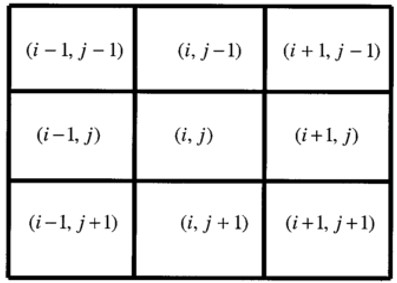
\includegraphics[width=0.6\textwidth]{figures/pixels.jpg}
	\caption{A 3x3 window illustration of the calculation of second difference of an (i,j) pixel \cite{Herraez2002}.}
	\label{fig:gammafactor}
\end{figure}


Unwrapping path is then defined by the reliability of an edge which is  the summation of the reliabilities of the pixels that the edge connects (either vertical or horizontal) and not just the reliability of the pixel. The unwrapping path then proceeds to unwrap the pixels with the highest edge reliability value first \cite{Herraez2002}. A flowchart and complete explanation of this algorithm is found in Appendix A.

This algorithm was already implemented in Python and available in the \texttt{scikit-image} library. The code was just modified to fit our desired results.

From the unwrapped phase maps, image processing techniques are further applied for enhancement of details which will be discussed in the following chapters.

\subsection{Phase To Height Conversion}

To determine the accuracy of the 3D reconstruction and the techniques applied, phase to height conversion is performed. We followed Du and Wang's algorithm \cite{Du2007}, explained in Appendix B, for phase to height conversion which only needs a reference object with varying depth/height measurements and particular number of points in it to obtain the actual depth/height.

A 5-step pyramid excluding the reference plane was used throughout the calibration since it has discrete height values.
